\documentclass[11pt, letterpaper]{article}

\usepackage{float}
\usepackage{csquotes}	% Recommended?
\usepackage{xcolor}		% color
\usepackage{subfigure}	% subfigure
\usepackage{graphicx}
\usepackage{amssymb}	% symbol
\usepackage{algorithm}	% algorithm
\usepackage{algpseudocode}
\usepackage{setspace}	% spacing
\usepackage{booktabs}	% table

\newcommand{\handout}[5]{
  \noindent
  \begin{center}
  \framebox{
    \vbox{
      \hbox to 5.78in { {\bf } \hfill #2 }
      \vspace{4mm}
      \hbox to 5.78in { {\Large \hfill #5  \hfill} }
      \vspace{2mm}
      \hbox to 5.78in { {\em #3 \hfill #4} }
    }
  }
  \end{center}
  \vspace*{4mm}
}
\newcommand{\lecture}[4]{\handout{#1}{#2}{#3}{#4}{#1}}

\newtheorem{theorem}{Theorem}
\newtheorem{corollary}[theorem]{Corollary}
\newtheorem{lemma}[theorem]{Lemma}
\newtheorem{observation}[theorem]{Observation}
\newtheorem{proposition}[theorem]{Proposition}
\newtheorem{definition}[theorem]{Definition}
\newtheorem{claim}[theorem]{Claim}
\newtheorem{fact}[theorem]{Fact}
\newtheorem{assumption}[theorem]{Assumption}
\topmargin 0pt
\advance \topmargin by -\headheight
\advance \topmargin by -\headsep
\textheight 9.5in
\oddsidemargin 0pt
\evensidemargin \oddsidemargin
\marginparwidth 0.5in
\textwidth 6.5in

\parindent 0in
\parskip 1.5ex

\begin{document}
\lecture{Programming Assignment 1 - Unfolding heuristics}{Spring 2016}{Yunjoo Park}{Computer Aided 3D Artifact Fabrication}


\section{Unfolding polytope}
Let \textit{P} be a polytope, bounded polyhedron. A simple polygon without overlapping is called \textit{net N} of \textit{P}. Each of polyhedra has multiple nets. The set of cut edges for the net is a spanning tree \textit{T}, the \textit{cut tree}, of \textit{G(P)}. An \textit{unfolding} is an isometric mappig \O : $F(P) \to {\mathbb{R}}^2 $ of the facets of $P$ to the Euclidean plane, such that for all $(f_1,f_2) \in D(P), \varphi(f_1)\cap \varphi(f_2)$ is an edge of both $\varphi(f_1)$ and $\varphi(f_2)$. $N(P,T) = \varphi(F(P))$ is the unfolding of \textit{P induced by T}. In this project, I will provide two implementation of unfolding heuristics from `Schlickenrieder, Wolfram. ``Net of Polyhedra." Master's Thesis, Technishe Universit$\ddot{a}$t Berlin (1997)' \cite{netpolyhedra}.
%In fact, there are two types of unfoldings. One is \textit{Edge unfolding}: Cut only along edges. The other is \textit{General unfoldings}: Cut through faces too. In this paper, I implement edge unfolding.


\section{Summary of four methods}
In this section, I will summarize four methods: 
\begin{itemize}
\item Steepest Edge Unfolding (SEU)
\item Flat Edge Unfolding (FEU)
\item Greatest increasing Edge Unfolding (GIU)
\item Rightmost ascending Edge Unfolding (REU)
\end{itemize}

Two methods, SEU and FEU, are given methods. I implement GIU and REU. \\
\\
An objective function $c$ is used in optimization; minimize or maximize.

\subsection{Steepest Edge Cut Tree}
If $c$ is an objective function in general position, let $v_-$ and $v_+$ be the bottom and top vertex of $P$ with regard to $c$. For each vertex except $v_+$, we choose the \textit{steepest ascending edge} at that vertex as a cut edge. This lead to straight paths from $v_-$ to $v_+$.

\begin{algorithm}
\caption{\textsc{Steepest-Edge-Unfold} ($P, c$)}\label{algo:steepest}
\begin{algorithmic}

	\State {\textsc{Initialize} $T = \emptyset $ }
    \For { \textbf{all vertices} $ v \in P,\ v \neq v_+ $}
		\State {\textit{Compute the steepest ascending edge incident to v (w.r.t. c),}}
        \State {\ \ \textit{ i.e. the edge e = (v,w), for which $\frac{\left\langle c, w-v \right\rangle}{\Vert w-v \Vert}$  is maximal.}}
        \State {$T = T \cup \left\{ e \right\}$}
        
    \EndFor
	\State {\Return{\textsc{Cut} $(P,T)$}}
\end{algorithmic}
\end{algorithm}

\subsection{Flat Edge Unfolding}
Let $c$ be a given vector. We join facets along \textit{flat} edges, which are as perpendicular as posible to the given vector $c$. Assign \textit{weights} to each edge $e^* \in D(P)$ where $e = (p,q)$  is the corresponding primal edge of $e^*$. Then compute a \textit{minimum spanning tree T} $D(P)$ with regard to these weights, and use this tree as the join tree.
For each vertex, we choose the \textit{steepest ascending edge} at that vertex as a cut edge.

\begin{algorithm}
\caption{\textsc{Flat-Spanning-Tree-Unfold} ($P, c$)}\label{algo:flat}
\begin{algorithmic}

	\State {\textsc{Initialize} $T = \emptyset $ }
    \For { \textbf{all edges} $ e = (p,q) \in P $}
		\State {\textit{let $e^*$ be the corresponding dual edge of e}}
        \State {\textit{let $ weights(e^*) =  \left| \frac{\left\langle c, p-q \right\rangle}{\Vert c \Vert \Vert p-q \Vert }\right|$}}      
    \EndFor
	\State {\textit{compute a minimal spanning tree T in D w.r.t. weights}}
	\State {\Return{\textsc{Join} $(P,T)$}}
\end{algorithmic}
\end{algorithm}



\subsection{Greatest Increase Cut Tree}
Let $c$ be an objective function in general position and $v_+$ the highest vertex. For each vertex except $v_+$, among all ascending edges incident to $v$, we choose the edge with \textit{greatest increasing} with regard to $c$. 

\begin{algorithm}
\caption{\textsc{Greatest-Increase-Unfold} ($P, c$)}\label{algo:greatest}
\begin{algorithmic}

	\State {\textsc{Initialize} $T = \emptyset $ }
    \For { \textbf{all vertices} $ v \in P,\ v \neq v_+ $}
		\State {\textit{Compute the edge with greatest increase (w.r.t. c) incident to v,}}
        \State {\ \ \textit{ i.e. the edge e = (v,w), for which $\left\langle c, w-v \right\rangle$  is maximal.}}
        \State {$T = T \cup \left\{ e \right\}$}
        
    \EndFor
	\State {\Return{\textsc{Cut} $(P,T)$}}
\end{algorithmic}
\end{algorithm}


\subsection{Rightmost Ascending Cut Tree}
Let $c$ be a vector in general position and $v_-$ the lowest and highest vertex of $P$ with regard to $c$. For each vertex $v \in V(P)$ except $v_-$, we ccompute the \textit{rightmost ascending edge} incident to $v$.
\begin{algorithm}
\caption{\textsc{Rightmost-Ascending-Edge-Unfold} ($P, c$)}\label{algo:rightmost}
\begin{algorithmic}
	\State {\textsc{Initialize} {$v\_ =$ the minimal vertex of $P$ w.r.t. $c$
    			\\ \ \ \ \ \ \ \ \ \ \ \ \ \ \ \ $b =$ the barycenter of $P$
                        \\ \ \ \ \ \ \ \ \ \ \ \ \ \ \ \ $T = \emptyset$}}
    \For { \textbf{all vertices} $ v \in P,\ v \neq v_- $}
		\State {\textit{let $e= (v,w)$ be the rightmost ascending edge incident to v,}}
        \State {\ \ \textit{ i.e. the edge, for which $\frac{\left\langle c, w-v \right\rangle}{\Vert w-v \Vert \Vert c \Vert} > 0$, and $ det(c, \frac{v-b}{\Vert v-b \Vert}, \frac{w-v}{\Vert w-v \Vert}) $ maximal.}}
        \State {$T = T \cup \left\{ e \right\}$}
    \EndFor
	\State {\Return{\textsc{Cut} $(P,T)$}}
\end{algorithmic}
\end{algorithm}

The barycenter of $P$ is the centroid of a polygon $P$. The centeroid of $P$ with uniform density can be computed as the weighted sum of the centroids of a partition of the polygon into triangles.
\begin{description}
  \item[First] Triangulate a polygon $P$.
  \item[Second] Compute the centroid of $P$.
	\begin{enumerate}
	  \item Form a sum of the centroids of each triangle, weighted by the area of each triangle.
	  \item Nomalize the whole sum by the total polyhedron.
	\end{enumerate}
  \item[Third] Create disks
\end{description}

%%%%%%%%%%%%%%%%%%%%%%%%%%%%%%%%%%%%%%%%%%%%%%%%%%%


\section{Results}
I test four heuristics methods on 5 convex models and 5 non-convex models.

%\section{Description of Models}

\subsection{Convex Models}
Shape of the models is as follows.
\begin{figure}[th]
\centering
%\subfigure[convex models]
{\includegraphics[height=0.4\textwidth]{FIGS/convex.jpg}}\hfill
\caption{The shape of convex models}
\label{fig:convex}
\end{figure}

The number of faces is as follows.
\begin{table}[th]
\centering
\caption{5 convex models}
\label{table:convex}
\begin{tabular}{@{}cccccc@{}}
\toprule
      & dioctagonal pyramid & tirakisicosahedron & cylinder & cube-03 & ball \\ \midrule
Faces & 32                  & 60                 & 140      & 108     & 760  \\ \bottomrule
\end{tabular}
\end{table}

%%%%%%%%%%%%%%%%%%%%%%%%%%%%%%%%%%%%%%%%%%%%%%%%%%%

\begin{figure*}[th]
\centering
\subfigure[model]
{\includegraphics[width=0.2\textwidth]{FIGS/s_pyramid.jpg}}
\hspace{5mm}
\subfigure[unfolded]
{\includegraphics[width=0.2\textwidth]{FIGS/convex/pyramid_s}}
\hspace{5mm}
\subfigure[cut]
{\includegraphics[width=0.2\textwidth]{FIGS/convex/pyramid_s_c}}
\hspace{5mm}
\subfigure[spanning tree]
{\includegraphics[width=0.2\textwidth]{FIGS/convex/pyramid_s_t}}
\hspace{5mm}
\caption{The Steepest Edge Unfold}
\end{figure*}

\begin{figure*}[h]
\centering
\subfigure[model]
{\includegraphics[height=0.2\textwidth]{FIGS/f_pyramid.jpg}}
\hspace{5mm}
\subfigure[unfolded]
{\includegraphics[width=0.2\textwidth]{FIGS/convex/pyramid_f}}
\hspace{5mm}
\subfigure[cut]
{\includegraphics[width=0.2\textwidth]{FIGS/convex/pyramid_f_c}}
\hspace{5mm}
\subfigure[spanning tree]
{\includegraphics[width=0.2\textwidth]{FIGS/convex/pyramid_f_t}}
\hspace{5mm}
\caption{The Flat Edge Unfold}
\end{figure*}

\begin{figure*}[h]
\centering
\subfigure[model]
{\includegraphics[width=0.2\textwidth]{FIGS/1_pyramid.jpg}}
\hspace{5mm}
\subfigure[unfolded]
{\includegraphics[width=0.2\textwidth]{FIGS/convex/pyramid_1}}
\hspace{5mm}
\subfigure[cut]
{\includegraphics[width=0.2\textwidth]{FIGS/convex/pyramid_1_c}}
\hspace{5mm}
\subfigure[spanning tree]
{\includegraphics[width=0.2\textwidth]{FIGS/convex/pyramid_1_t}}
\hspace{5mm}
\caption{The Greatest Increase Unfold}
\end{figure*}


\begin{figure*}[h]
\centering
\subfigure[model]
{\includegraphics[width=0.2\textwidth]{FIGS/2_pyramid.jpg}}
\hspace{5mm}
\subfigure[unfolded]
{\includegraphics[width=0.2\textwidth]{FIGS/convex/pyramid_2}}
\hspace{5mm}
\subfigure[cut]
{\includegraphics[width=0.2\textwidth]{FIGS/convex/pyramid_2_c}}
\hspace{5mm}
\subfigure[spanning tree]
{\includegraphics[width=0.2\textwidth]{FIGS/convex/pyramid_2_t}}
\hspace{5mm}
\caption{The Rightemost Ascending Edge Unfold}
\end{figure*}
%%%%%%%%%%%%%%%%%%%%%%%%%%%%%%%%%%%%%%%%%%%%%%%%%%%

%%%%%%%%%%%%%%%%%%%%%%%%%%%%%%%%%%%%%%%%%%%%%%%%%%%
\begin{figure*}[th]
\centering
\subfigure[model]
{\includegraphics[width=0.2\textwidth]{FIGS/s_icosa.jpg}}
\hspace{5mm}
\subfigure[unfolded]
{\includegraphics[width=0.2\textwidth]{FIGS/convex/icosa_s}}
\hspace{5mm}
\subfigure[cut]
{\includegraphics[width=0.2\textwidth]{FIGS/convex/icosa_s_c}}
\hspace{5mm}
\subfigure[spanning tree]
{\includegraphics[width=0.2\textwidth]{FIGS/convex/icosa_s_t}}
\hspace{5mm}
\caption{The Steepest Edge Unfold}
\end{figure*}

\begin{figure*}[h]
\centering
\subfigure[model]
{\includegraphics[width=0.2\textwidth]{FIGS/f_icosa.jpg}}
\hspace{5mm}
\subfigure[unfolded]
{\includegraphics[width=0.2\textwidth]{FIGS/convex/icosa_f}}
\hspace{5mm}
\subfigure[cut]
{\includegraphics[width=0.2\textwidth]{FIGS/convex/icosa_f_c}}
\hspace{5mm}
\subfigure[spanning tree]
{\includegraphics[width=0.2\textwidth]{FIGS/convex/icosa_f_t}}
\hspace{5mm}
\caption{The Flat Edge Unfold}
\end{figure*}

\begin{figure*}[h]
\centering
\subfigure[model]
{\includegraphics[width=0.2\textwidth]{FIGS/1_icosa.jpg}}
\hspace{5mm}
\subfigure[unfolded]
{\includegraphics[width=0.2\textwidth]{FIGS/convex/icosa_1}}
\hspace{5mm}
\subfigure[cut]
{\includegraphics[width=0.2\textwidth]{FIGS/convex/icosa_1_c}}
\hspace{5mm}
\subfigure[spanning tree]
{\includegraphics[width=0.2\textwidth]{FIGS/convex/icosa_1_t}}
\hspace{5mm}
\caption{The Greatest Increase Unfold}
\end{figure*}


\begin{figure*}[h]
\centering
\subfigure[model]
{\includegraphics[width=0.2\textwidth]{FIGS/2_icosa.jpg}}
\hspace{5mm}
\subfigure[unfolded]
{\includegraphics[width=0.2\textwidth]{FIGS/convex/icosa_2}}
\hspace{5mm}
\subfigure[cut]
{\includegraphics[width=0.2\textwidth]{FIGS/convex/icosa_2_c}}
\hspace{5mm}
\subfigure[spanning tree]
{\includegraphics[width=0.2\textwidth]{FIGS/convex/icosa_2_t}}
\hspace{5mm}
\caption{The Rightemost Ascending Edge Unfold}
\end{figure*}
%%%%%%%%%%%%%%%%%%%%%%%%%%%%%%%%%%%%%%%%%%%%%%%%%%%

%%%%%%%%%%%%%%%%%%%%%%%%%%%%%%%%%%%%%%%%%%%%%%%%%%%
\begin{figure*}[th]
\centering
\subfigure[model]
{\includegraphics[width=0.2\textwidth]{FIGS/s_cylinder.jpg}}
\hspace{5mm}
\subfigure[unfolded]
{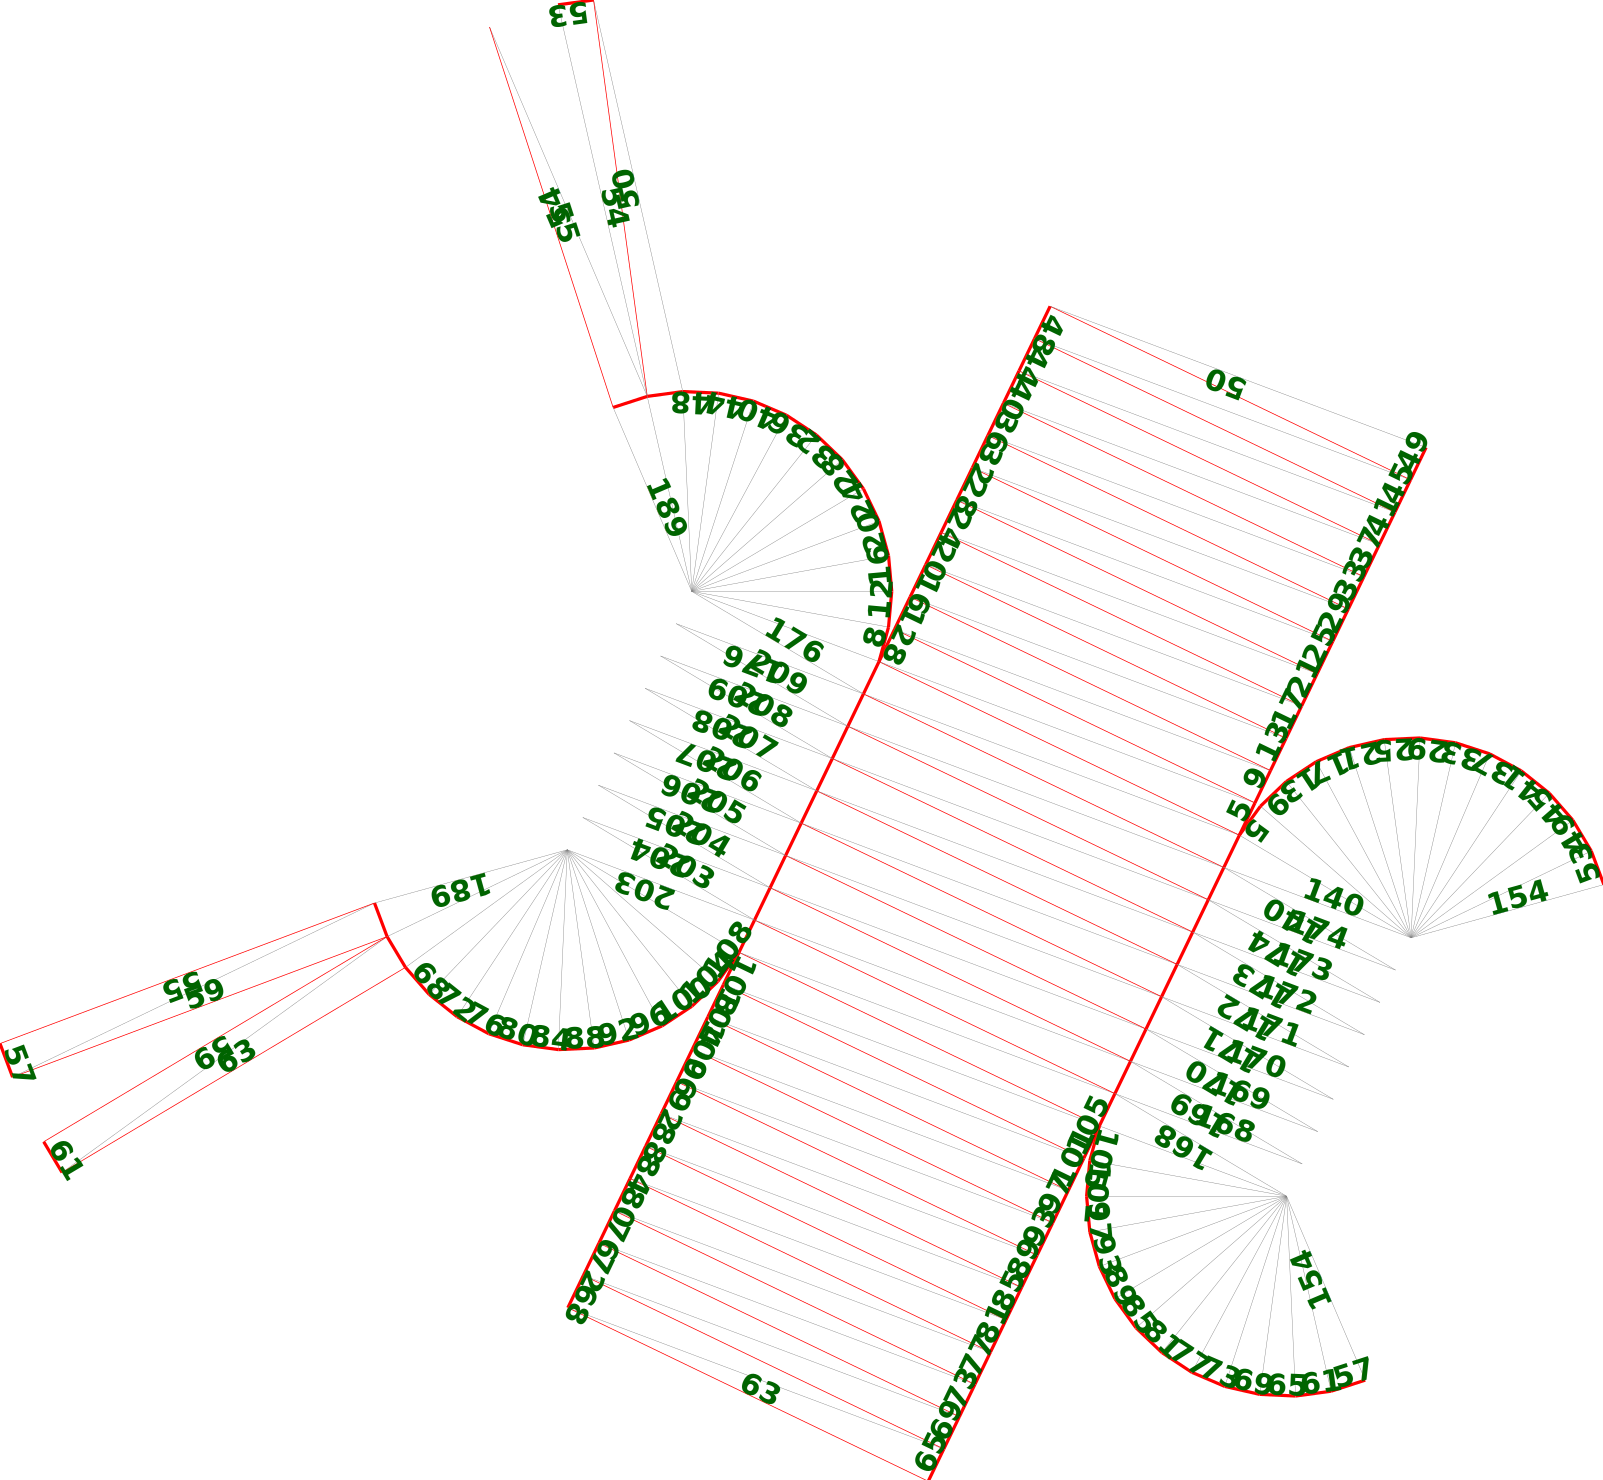
\includegraphics[width=0.2\textwidth]{FIGS/convex/cylinder_s}}
\hspace{5mm}
\subfigure[cut]
{\includegraphics[width=0.2\textwidth]{FIGS/convex/cylinder_s_c}}
\hspace{5mm}
\subfigure[spanning tree]
{\includegraphics[width=0.2\textwidth]{FIGS/convex/cylinder_s_t}}
\hspace{5mm}
\caption{The Steepest Edge Unfold}
\end{figure*}

\begin{figure*}[h]
\centering
\subfigure[model]
{\includegraphics[width=0.2\textwidth]{FIGS/f_cylinder.jpg}}
\hspace{5mm}
\subfigure[unfolded]
{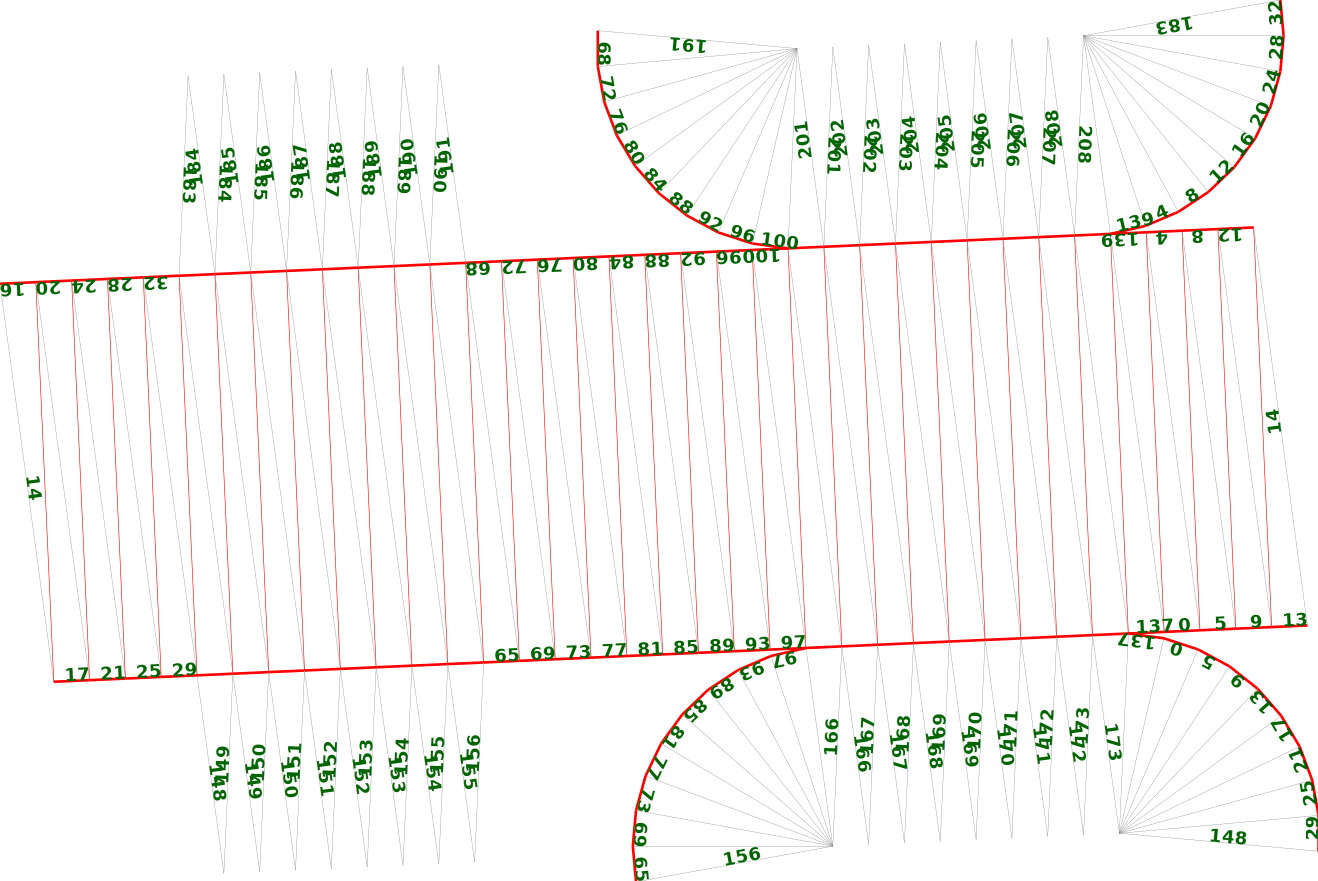
\includegraphics[width=0.2\textwidth]{FIGS/convex/cylinder_f}}
\hspace{5mm}
\subfigure[cut]
{\includegraphics[width=0.2\textwidth]{FIGS/convex/cylinder_f_c}}
\hspace{5mm}
\subfigure[spanning tree]
{\includegraphics[width=0.2\textwidth]{FIGS/convex/cylinder_f_t}}
\hspace{5mm}
\caption{The Flat Edge Unfold}
\end{figure*}

\begin{figure*}[h]
\centering
\subfigure[model]
{\includegraphics[width=0.2\textwidth]{FIGS/1_cylinder.jpg}}
\hspace{5mm}
\subfigure[unfolded]
{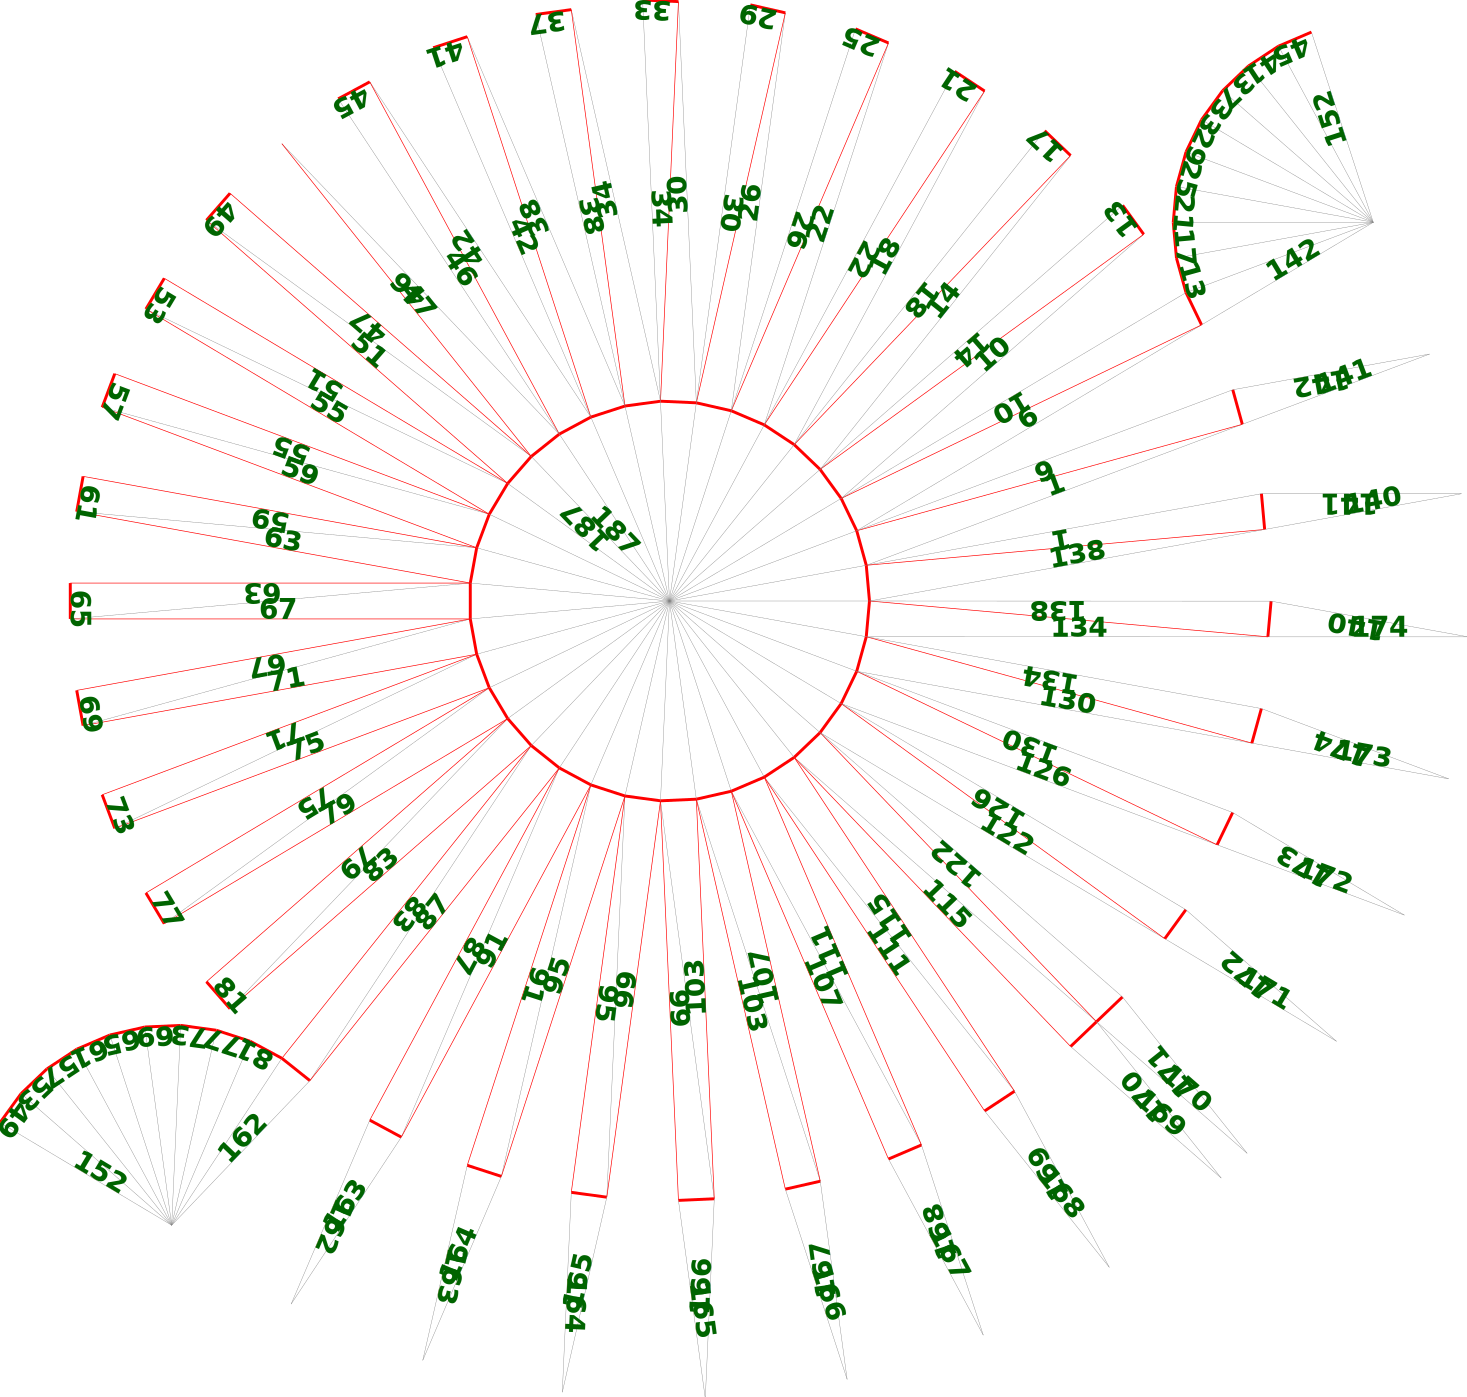
\includegraphics[width=0.2\textwidth]{FIGS/convex/cylinder_1}}
\hspace{5mm}
\subfigure[cut]
{\includegraphics[width=0.2\textwidth]{FIGS/convex/cylinder_1_c}}
\hspace{5mm}
\subfigure[spanning tree]
{\includegraphics[width=0.2\textwidth]{FIGS/convex/cylinder_1_t}}
\hspace{5mm}
\caption{The Greatest Increase Unfold}
\end{figure*}


\begin{figure*}[h]
\centering
\subfigure[model]
{\includegraphics[width=0.2\textwidth]{FIGS/2_cylinder.jpg}}
\hspace{5mm}
\subfigure[unfolded]
{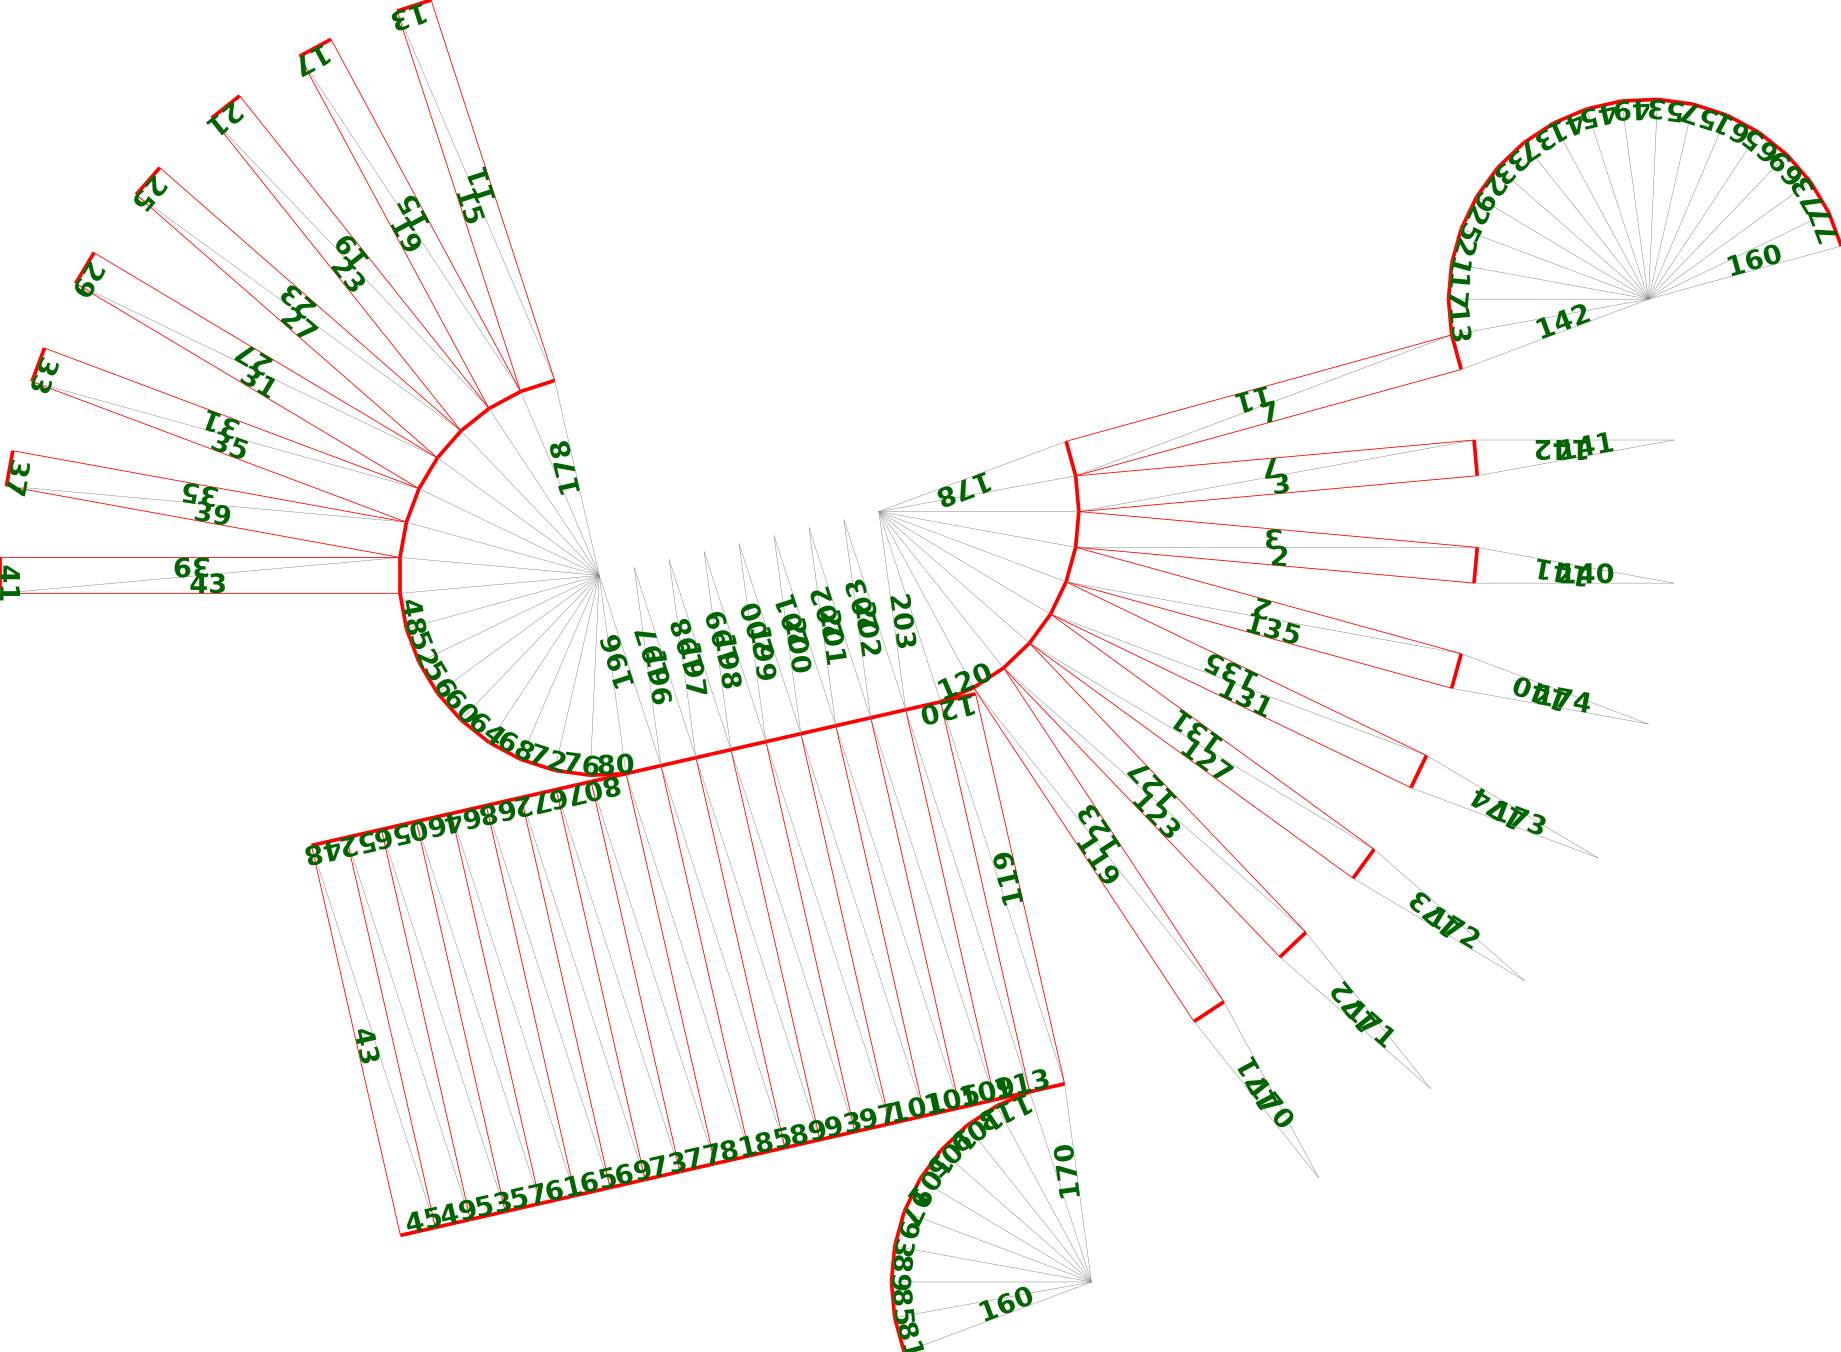
\includegraphics[width=0.2\textwidth]{FIGS/convex/cylinder_2}}
\hspace{5mm}
\subfigure[cut]
{\includegraphics[width=0.2\textwidth]{FIGS/convex/cylinder_2_c}}
\hspace{5mm}
\subfigure[spanning tree]
{\includegraphics[width=0.2\textwidth]{FIGS/convex/cylinder_2_t}}
\hspace{5mm}
\caption{The Rightemost Ascending Edge Unfold}
\end{figure*}
%%%%%%%%%%%%%%%%%%%%%%%%%%%%%%%%%%%%%%%%%%%%%%%%%%%
\begin{figure*}[th]
\centering
\subfigure[model]
{\includegraphics[width=0.2\textwidth]{FIGS/s_cube.jpg}}
\hspace{5mm}
\subfigure[unfolded]
{\includegraphics[height=0.2\textwidth]{FIGS/convex/cube-03_s}}
\hspace{5mm}
\subfigure[cut]
{\includegraphics[height=0.2\textwidth]{FIGS/convex/cube-03_s_c}}
\hspace{5mm}
\subfigure[spanning tree]
{\includegraphics[height=0.2\textwidth]{FIGS/convex/cube-03_s_t}}
\hspace{5mm}
\caption{The Steepest Edge Unfold}
\end{figure*}

\begin{figure*}[h]
\centering
\subfigure[model]
{\includegraphics[width=0.2\textwidth]{FIGS/f_cube.jpg}}
\hspace{5mm}
\subfigure[unfolded]
{\includegraphics[width=0.15\textwidth]{FIGS/convex/cube-03_f}}
\hspace{5mm}
\subfigure[cut]
{\includegraphics[width=0.15\textwidth]{FIGS/convex/cube-03_f_c}}
\hspace{5mm}
\subfigure[spanning tree]
{\includegraphics[width=0.15\textwidth]{FIGS/convex/cube-03_f_t}}
\hspace{5mm}
\caption{The Flat Edge Unfold}
\end{figure*}

\begin{figure*}[h]
\centering
\subfigure[model]
{\includegraphics[width=0.2\textwidth]{FIGS/1_cube.jpg}}
\hspace{5mm}
\subfigure[unfolded]
{\includegraphics[height=0.2\textwidth]{FIGS/convex/cube-03_1}}
\hspace{5mm}
\subfigure[cut]
{\includegraphics[height=0.2\textwidth]{FIGS/convex/cube-03_1_c}}
\hspace{5mm}
\subfigure[spanning tree]
{\includegraphics[height=0.2\textwidth]{FIGS/convex/cube-03_1_t}}
\hspace{5mm}
\caption{The Greatest Increase Unfold}
\end{figure*}


\begin{figure*}[h]
\centering
\subfigure[model]
{\includegraphics[width=0.2\textwidth]{FIGS/2_cube.jpg}}
\hspace{5mm}
\subfigure[unfolded]
{\includegraphics[width=0.2\textwidth]{FIGS/convex/cube-03_2}}
\hspace{5mm}
\subfigure[cut]
{\includegraphics[width=0.2\textwidth]{FIGS/convex/cube-03_2_c}}
\hspace{5mm}
\subfigure[spanning tree]
{\includegraphics[width=0.2\textwidth]{FIGS/convex/cube-03_2_t}}
\hspace{5mm}
\caption{The Rightemost Ascending Edge Unfold}
\end{figure*}
%%%%%%%%%%%%%%%%%%%%%%%%%%%%%%%%%%%%%%%%%%%%%%%%%%%

%%%%%%%%%%%%%%%%%%%%%%%%%%%%%%%%%%%%%%%%%%%%%%%%%%%
\begin{figure*}[th]
\centering
\subfigure[model]
{\includegraphics[width=0.2\textwidth]{FIGS/s_ball.jpg}}
\hspace{5mm}
\subfigure[unfolded]
{\includegraphics[width=0.2\textwidth]{FIGS/convex/ball_s}}
\hspace{5mm}
\subfigure[cut]
{\includegraphics[width=0.2\textwidth]{FIGS/convex/ball_s_c}}
\hspace{5mm}
\subfigure[spanning tree]
{\includegraphics[width=0.2\textwidth]{FIGS/convex/ball_s_t}}
\hspace{5mm}
\caption{The Steepest Edge Unfold}
\end{figure*}

\begin{figure*}[h]
\centering
\subfigure[model]
{\includegraphics[width=0.2\textwidth]{FIGS/f_ball.jpg}}
\hspace{5mm}
\subfigure[unfolded]
{\includegraphics[width=0.22\textwidth]{FIGS/convex/ball_f}}
\hspace{5mm}
\subfigure[cut]
{\includegraphics[width=0.22\textwidth]{FIGS/convex/ball_f_c}}
\hspace{5mm}
\subfigure[spanning tree]
{\includegraphics[width=0.22\textwidth]{FIGS/convex/ball_f_t}}
\hspace{5mm}
\caption{The Flat Edge Unfold}
\end{figure*}

\begin{figure*}[h]
\centering
\subfigure[model]
{\includegraphics[width=0.2\textwidth]{FIGS/1_ball.jpg}}
\hspace{5mm}
\subfigure[unfolded]
{\includegraphics[width=0.2\textwidth]{FIGS/convex/ball_1}}
\hspace{5mm}
\subfigure[cut]
{\includegraphics[width=0.2\textwidth]{FIGS/convex/ball_1_c}}
\hspace{5mm}
\subfigure[spanning tree]
{\includegraphics[width=0.2\textwidth]{FIGS/convex/ball_1_t}}
\hspace{5mm}
\caption{The Greatest Increase Unfold}
\end{figure*}


\begin{figure*}[h]
\centering
\subfigure[model]
{\includegraphics[width=0.2\textwidth]{FIGS/2_ball.jpg}}
\hspace{5mm}
\subfigure[unfolded]
{\includegraphics[width=0.2\textwidth]{FIGS/convex/ball_2}}
\hspace{5mm}
\subfigure[cut]
{\includegraphics[width=0.2\textwidth]{FIGS/convex/ball_2_c}}
\hspace{5mm}
\subfigure[spanning tree]
{\includegraphics[width=0.2\textwidth]{FIGS/convex/ball_2_t}}
\hspace{5mm}
\caption{The Rightemost Ascending Edge Unfold}
\end{figure*}
%%%%%%%%%%%%%%%%%%%%%%%%%%%%%%%%%%%%%%%%%%%%%%%%%%%

%%%%%%%%%%%%%%%%%%%%%%%%%%%%%%%%%%%%%%%%%%%%%%%%%%%
\clearpage
\subsection{non-Convex Models}
Shape of the models is as follows.
\begin{figure}[th]
\centering
{\includegraphics[height=0.4\textwidth]{FIGS/nonconvex.jpg}}
\caption{The shape of non-convexx models}
\label{fig:nonconvex}
\end{figure}

The number of faces is as follows.
\begin{table}[th]
\centering
\caption{5 non-convex models}
\label{table:nonconvex}
\begin{tabular}{@{}cccccc@{}}
\toprule
      & DwarfAxeMan & knot & pooh & mushroom & star-4split \\ \midrule
Faces & 1000        & 480  & 392  & 200      & 96          \\ \bottomrule
\end{tabular}
\end{table}
\\
Unlike testing on convex models, unfolding a non-convex model requires many attempts. There is a $-r \ \ n$ option. It implies that it attempts at most $n$ times until the mesh is unfolded without overlapping. Especially, I tried 1000 times.


%%%%%%%%%%%%%%%%%%%%%%%%%%%%%%%%%%%%%%%%%%%%%%%%%%%
\begin{itemize}
	\item \textsc{Dwarf Axe Man}
	\\All mehtods have similar number of overlapping. Compared to other three methods, the rightmost ascending edge unfolding method takes more time.
	\item \textsc{Knot}
	\\All methods cannot generate a unfolded polygon without overlapping. They take similar time and generate similar number of overlappings.
	\item \textsc{Pooh}
	\\The rightmost ascending edge unfolding method takes a little more time. All methods fail to generate unfolded polygon without overlappings.
	\item \textsc{Mushroom}
	\\The steepest edge unfolding methods has the smallest number of overlappings in $min/avg/max$ overlaps.
	\item \textsc{Star-4split}
	\\Only the rightmost ascending edge unfolding method generates unfolded polygon without overlapping. The method completed unfolding $star$ model with only 7 times.
\end{itemize}

	
\begin{figure*}[th]
\centering
\subfigure[model]
{\includegraphics[width=0.2\textwidth]{FIGS/s_dwarf.jpg}}
\hspace{5mm}
\subfigure[unfolded]
{\includegraphics[width=0.2\textwidth]{FIGS/nonconvex/n_DwarfAxeMan_s}}
\hspace{5mm}
\subfigure[cut]
{\includegraphics[width=0.2\textwidth]{FIGS/nonconvex/n_DwarfAxeMan_s_c}}
\hspace{5mm}
\subfigure[spanning tree]
{\includegraphics[width=0.2\textwidth]{FIGS/nonconvex/n_DwarfAxeMan_s_t}}
\hspace{5mm}
\caption{The Steepest Edge Unfold}
\end{figure*}

\begin{figure*}[h]
\centering
\subfigure[model]
{\includegraphics[width=0.2\textwidth]{FIGS/f_dwarf.jpg}}
\hspace{5mm}
\subfigure[unfolded]
{\includegraphics[width=0.2\textwidth]{FIGS/nonconvex/n_DwarfAxeMan_f}}
\hspace{5mm}
\subfigure[cut]
{\includegraphics[width=0.2\textwidth]{FIGS/nonconvex/n_DwarfAxeMan_f_c}}
\hspace{5mm}
\subfigure[spanning tree]
{\includegraphics[width=0.2\textwidth]{FIGS/nonconvex/n_DwarfAxeMan_f_t}}
\hspace{5mm}
\caption{The Flat Edge Unfold}
\end{figure*}

\begin{figure*}[h]
\centering
\subfigure[model]
{\includegraphics[width=0.2\textwidth]{FIGS/1_dwarf.jpg}}
\hspace{5mm}
\subfigure[unfolded]
{\includegraphics[width=0.2\textwidth]{FIGS/nonconvex/n_DwarfAxeMan_1}}
\hspace{5mm}
\subfigure[cut]
{\includegraphics[width=0.2\textwidth]{FIGS/nonconvex/n_DwarfAxeMan_1_c}}
\hspace{5mm}
\subfigure[spanning tree]
{\includegraphics[width=0.2\textwidth]{FIGS/nonconvex/n_DwarfAxeMan_1_t}}
\hspace{5mm}
\caption{The Greatest Increase Unfold}
\end{figure*}


\begin{figure*}[h]
\centering
\subfigure[model]
{\includegraphics[width=0.2\textwidth]{FIGS/2_dwarf.jpg}}
\hspace{5mm}
\subfigure[unfolded]
{\includegraphics[width=0.2\textwidth]{FIGS/nonconvex/n_DwarfAxeMan_2}}
\hspace{5mm}
\subfigure[cut]
{\includegraphics[width=0.2\textwidth]{FIGS/nonconvex/n_DwarfAxeMan_2_c}}
\hspace{5mm}
\subfigure[spanning tree]
{\includegraphics[width=0.2\textwidth]{FIGS/nonconvex/n_DwarfAxeMan_2_t}}
\hspace{5mm}
\caption{The Rightemost Ascending Edge Unfold}
\end{figure*}
%%%%%%%%%%%%%%%%%%%%%%%%%%%%%%%%%%%%%%%%%%%%%%%%%%%

%%%%%%%%%%%%%%%%%%%%%%%%%%%%%%%%%%%%%%%%%%%%%%%%%%%
\begin{figure*}[th]
\centering
\subfigure[model]
{\includegraphics[width=0.2\textwidth]{FIGS/s_knot.jpg}}
\hspace{5mm}
\subfigure[unfolded]
{\includegraphics[width=0.2\textwidth]{FIGS/nonconvex/n_knot_s}}
\hspace{5mm}
\subfigure[cut]
{\includegraphics[width=0.2\textwidth]{FIGS/nonconvex/n_knot_s_c}}
\hspace{5mm}
\subfigure[spanning tree]
{\includegraphics[width=0.2\textwidth]{FIGS/nonconvex/n_knot_s_t}}
\hspace{5mm}
\caption{The Steepest Edge Unfold}
\end{figure*}

\begin{figure*}[h]
\centering
\subfigure[model]
{\includegraphics[width=0.2\textwidth]{FIGS/f_knot.jpg}}
\hspace{5mm}
\subfigure[unfolded]
{\includegraphics[width=0.2\textwidth]{FIGS/nonconvex/n_knot_f}}
\hspace{5mm}
\subfigure[cut]
{\includegraphics[width=0.2\textwidth]{FIGS/nonconvex/n_knot_f_c}}
\hspace{5mm}
\subfigure[spanning tree]
{\includegraphics[width=0.2\textwidth]{FIGS/nonconvex/n_knot_f_t}}
\hspace{5mm}
\caption{The Flat Edge Unfold}
\end{figure*}

\begin{figure*}[h]
\centering
\subfigure[model]
{\includegraphics[width=0.2\textwidth]{FIGS/1_knot.jpg}}
\hspace{5mm}
\subfigure[unfolded]
{\includegraphics[width=0.2\textwidth]{FIGS/nonconvex/n_knot_1}}
\hspace{5mm}
\subfigure[cut]
{\includegraphics[width=0.2\textwidth]{FIGS/nonconvex/n_knot_1_c}}
\hspace{5mm}
\subfigure[spanning tree]
{\includegraphics[width=0.2\textwidth]{FIGS/nonconvex/n_knot_1_t}}
\hspace{5mm}
\caption{The Greatest Increase Unfold}
\end{figure*}


\begin{figure*}[h]
\centering
\subfigure[model]
{\includegraphics[width=0.2\textwidth]{FIGS/2_knot.jpg}}
\hspace{5mm}
\subfigure[unfolded]
{\includegraphics[width=0.2\textwidth]{FIGS/nonconvex/n_knot_2}}
\hspace{5mm}
\subfigure[cut]
{\includegraphics[width=0.2\textwidth]{FIGS/nonconvex/n_knot_2_c}}
\hspace{5mm}
\subfigure[spanning tree]
{\includegraphics[width=0.2\textwidth]{FIGS/nonconvex/n_knot_2_t}}
\hspace{5mm}
\caption{The Rightemost Ascending Edge Unfold}
\end{figure*}
%%%%%%%%%%%%%%%%%%%%%%%%%%%%%%%%%%%%%%%%%%%%%%%%%%%



%%%%%%%%%%%%%%%%%%%%%%%%%%%%%%%%%%%%%%%%%%%%%%%%%%%
\begin{figure*}[th]
\centering
\subfigure[model]
{\includegraphics[width=0.2\textwidth]{FIGS/s_pooh.jpg}}
\hspace{5mm}
\subfigure[unfolded]
{\includegraphics[width=0.2\textwidth]{FIGS/nonconvex/n_pooh_s}}
\hspace{5mm}
\subfigure[cut]
{\includegraphics[width=0.2\textwidth]{FIGS/nonconvex/n_pooh_s_c}}
\hspace{5mm}
\subfigure[spanning tree]
{\includegraphics[width=0.2\textwidth]{FIGS/nonconvex/n_pooh_s_t}}
\hspace{5mm}
\caption{The Steepest Edge Unfold}
\end{figure*}

\begin{figure*}[h]
\centering
\subfigure[model]
{\includegraphics[width=0.2\textwidth]{FIGS/f_pooh.jpg}}
\hspace{5mm}
\subfigure[unfolded]
{\includegraphics[width=0.2\textwidth]{FIGS/nonconvex/n_pooh_f}}
\hspace{5mm}
\subfigure[cut]
{\includegraphics[width=0.2\textwidth]{FIGS/nonconvex/n_pooh_f_c}}
\hspace{5mm}
\subfigure[spanning tree]
{\includegraphics[width=0.2\textwidth]{FIGS/nonconvex/n_pooh_f_t}}
\hspace{5mm}
\caption{The Flat Edge Unfold}
\end{figure*}

\begin{figure*}[h]
\centering
\subfigure[model]
{\includegraphics[width=0.2\textwidth]{FIGS/1_pooh.jpg}}
\hspace{5mm}
\subfigure[unfolded]
{\includegraphics[width=0.2\textwidth]{FIGS/nonconvex/n_pooh_1}}
\hspace{5mm}
\subfigure[cut]
{\includegraphics[width=0.2\textwidth]{FIGS/nonconvex/n_pooh_1_c}}
\hspace{5mm}
\subfigure[spanning tree]
{\includegraphics[width=0.2\textwidth]{FIGS/nonconvex/n_pooh_1_t}}
\hspace{5mm}
\caption{The Greatest Increase Unfold}
\end{figure*}


\begin{figure*}[h]
\centering
\subfigure[model]
{\includegraphics[width=0.2\textwidth]{FIGS/2_pooh.jpg}}
\hspace{5mm}
\subfigure[unfolded]
{\includegraphics[width=0.2\textwidth]{FIGS/nonconvex/n_pooh_2}}
\hspace{5mm}
\subfigure[cut]
{\includegraphics[width=0.2\textwidth]{FIGS/nonconvex/n_pooh_2_c}}
\hspace{5mm}
\subfigure[spanning tree]
{\includegraphics[width=0.2\textwidth]{FIGS/nonconvex/n_pooh_2_t}}
\hspace{5mm}
\caption{The Rightemost Ascending Edge Unfold}
\end{figure*}
%%%%%%%%%%%%%%%%%%%%%%%%%%%%%%%%%%%%%%%%%%%%%%%%%%%



%%%%%%%%%%%%%%%%%%%%%%%%%%%%%%%%%%%%%%%%%%%%%%%%%%%
\begin{figure*}[th]
\centering
\subfigure[model]
{\includegraphics[width=0.2\textwidth]{FIGS/s_mushroom.jpg}}
\hspace{5mm}
\subfigure[unfolded]
{\includegraphics[width=0.2\textwidth]{FIGS/nonconvex/n_mushroom_s}}
\hspace{5mm}
\subfigure[cut]
{\includegraphics[width=0.2\textwidth]{FIGS/nonconvex/n_mushroom_s_c}}
\hspace{5mm}
\subfigure[spanning tree]
{\includegraphics[width=0.2\textwidth]{FIGS/nonconvex/n_mushroom_s_t}}
\hspace{5mm}
\caption{The Steepest Edge Unfold}
\end{figure*}

\begin{figure*}[h]
\centering
\subfigure[model]
{\includegraphics[width=0.2\textwidth]{FIGS/f_mushroom.jpg}}
\hspace{5mm}
\subfigure[unfolded]
{\includegraphics[width=0.2\textwidth]{FIGS/nonconvex/n_mushroom_f}}
\hspace{5mm}
\subfigure[cut]
{\includegraphics[width=0.2\textwidth]{FIGS/nonconvex/n_mushroom_f_c}}
\hspace{5mm}
\subfigure[spanning tree]
{\includegraphics[width=0.2\textwidth]{FIGS/nonconvex/n_mushroom_f_t}}
\hspace{5mm}
\caption{The Flat Edge Unfold}
\end{figure*}

\begin{figure*}[h]
\centering
\subfigure[model]
{\includegraphics[width=0.2\textwidth]{FIGS/1_mushroom.jpg}}
\hspace{5mm}
\subfigure[unfolded]
{\includegraphics[width=0.2\textwidth]{FIGS/nonconvex/n_mushroom_1}}
\hspace{5mm}
\subfigure[cut]
{\includegraphics[width=0.2\textwidth]{FIGS/nonconvex/n_mushroom_1_c}}
\hspace{5mm}
\subfigure[spanning tree]
{\includegraphics[width=0.2\textwidth]{FIGS/nonconvex/n_mushroom_1_t}}
\hspace{5mm}
\caption{The Greatest Increase Unfold}
\end{figure*}


\begin{figure*}[ht]
\centering
\subfigure[model]
{\includegraphics[width=0.2\textwidth]{FIGS/2_mushroom.jpg}}
\hspace{5mm}
\subfigure[unfolded]
{\includegraphics[width=0.2\textwidth]{FIGS/nonconvex/mushroom_2.jpg}}
\hspace{5mm}
\subfigure[cut]
{\includegraphics[width=0.2\textwidth]{FIGS/nonconvex/mushroom_2_c.jpg}}
\hspace{5mm}
\subfigure[spanning tree]
{\includegraphics[width=0.2\textwidth]{FIGS/nonconvex/mushroom_2_t.jpg}}
\hspace{5mm}
\caption{The Rightemost Ascending Edge Unfold}
\end{figure*}
%%%%%%%%%%%%%%%%%%%%%%%%%%%%%%%%%%%%%%%%%%%%%%%%%%%



%%%%%%%%%%%%%%%%%%%%%%%%%%%%%%%%%%%%%%%%%%%%%%%%%%%
\begin{figure*}[th]
\centering
\subfigure[model]
{\includegraphics[width=0.2\textwidth]{FIGS/s_star.jpg}}
\hspace{5mm}
\subfigure[unfolded]
{\includegraphics[width=0.2\textwidth]{FIGS/nonconvex/n_star_s}}
\hspace{5mm}
\subfigure[cut]
{\includegraphics[width=0.2\textwidth]{FIGS/nonconvex/n_star_s_c}}
\hspace{5mm}
\subfigure[spanning tree]
{\includegraphics[width=0.2\textwidth]{FIGS/nonconvex/n_star_s_t}}
\hspace{5mm}
\caption{The Steepest Edge Unfold}
\end{figure*}

\begin{figure*}[h]
\centering
\subfigure[model]
{\includegraphics[width=0.2\textwidth]{FIGS/f_star.jpg}}
\hspace{5mm}
\subfigure[unfolded]
{\includegraphics[width=0.2\textwidth]{FIGS/nonconvex/n_star_f}}
\hspace{5mm}
\subfigure[cut]
{\includegraphics[width=0.2\textwidth]{FIGS/nonconvex/n_star_f_c}}
\hspace{5mm}
\subfigure[spanning tree]
{\includegraphics[width=0.2\textwidth]{FIGS/nonconvex/n_star_f_t}}
\hspace{5mm}
\caption{The Flat Edge Unfold}
\end{figure*}

\begin{figure*}[h]
\centering
\subfigure[model]
{\includegraphics[width=0.2\textwidth]{FIGS/1_star.jpg}}
\hspace{5mm}
\subfigure[unfolded]
{\includegraphics[width=0.2\textwidth]{FIGS/nonconvex/n_star_1}}
\hspace{5mm}
\subfigure[cut]
{\includegraphics[width=0.2\textwidth]{FIGS/nonconvex/n_star_1_c}}
\hspace{5mm}
\subfigure[spanning tree]
{\includegraphics[width=0.2\textwidth]{FIGS/nonconvex/n_star_1_t}}
\hspace{5mm}
\caption{The Greatest Increase Unfold}
\end{figure*}


\begin{figure*}[h]
\centering
\subfigure[model]
{\includegraphics[width=0.2\textwidth]{FIGS/2_star.jpg}}
\hspace{5mm}
\subfigure[unfolded]
{\includegraphics[width=0.2\textwidth]{FIGS/nonconvex/n_star_2}}
\hspace{5mm}
\subfigure[cut]
{\includegraphics[width=0.2\textwidth]{FIGS/nonconvex/n_star_2_c}}
\hspace{5mm}
\subfigure[spanning tree]
{\includegraphics[width=0.2\textwidth]{FIGS/nonconvex/n_star_2_t}}
\hspace{5mm}
\caption{The Rightemost Ascending Edge Unfold}
\end{figure*}



%%%%%%%%%%%%%%%%%%%%%%%%%%%%%%%%%%%%%%%%%%%%%%%%%%%

\clearpage
\section{Foundings}
Since I use a random vector $c$ with $\Vert c \Vert = 1$, I do not care about length. Although four methods do not work well for non-convex model, they successfully generate unfolded polygons for convex models. 
\begin{itemize}
	\item{Time}
	\\All methods take similar amount of time. However, the rightmost ascendiing edge unfold method takes more time with a complicated model.
	\item{Overlapping}
	\\The flat edge unfold method has much more than the others.
	\item{Height}
	\\The height of tree of the rightmost ascending edge is higher than the others.
\end{itemize}


\section{GUI Options}
It is possible to change back color of unfolded polygons.
\begin{figure*}[th]
\centering
\includegraphics[width=0.2\textwidth]{FIGS/triakisicosahedron_s-wi-green.jpg}
\hspace{5mm}
\includegraphics[width=0.2\textwidth]{FIGS/triakisicosahedron_s-wi-mint.jpg}
\hspace{5mm}
\includegraphics[width=0.2\textwidth]{FIGS/triakisicosahedron_s-wi-ppink.jpg}
\hspace{5mm}
\includegraphics[width=0.2\textwidth]{FIGS/triakisicosahedron_s-wi-skyblue.jpg}
\caption{Triakisicosahedron using the steepest edge unfold method}
\end{figure*}

It is possible to generate a unfolded polygon randomly.
\begin{figure*}[th]
\centering
\includegraphics[width=0.2\textwidth]{FIGS/dioctagonal_pyramid_s1.jpg}
\hspace{5mm}
\includegraphics[width=0.2\textwidth]{FIGS/dioctagonal_pyramid_s2.jpg}
\hspace{5mm}
\includegraphics[width=0.2\textwidth]{FIGS/dioctagonal_pyramid_s3.jpg}
\hspace{5mm}
\includegraphics[width=0.2\textwidth]{FIGS/dioctagonal_pyramid_s4.jpg}
\caption{Dioctagonal pyramid using the steepest edge unfold method}
\end{figure*}

% \begin{figure*}[th]
% \centering
% \subfigure[The Steepest Edge Unfold]
% {\includegraphics[width=0.4\textwidth]{FIGS/dwarf_s_cmd.jpg}}
% \hspace{5mm}
% \subfigure[Flat Edge Unfold]
% {\includegraphics[width=0.4\textwidth]{FIGS/dwarf_f_cmd.jpg}}
% \subfigure[The Greatest Increase Edge Unfold]
% {\includegraphics[width=0.4\textwidth]{FIGS/dwarf_1_cmd.jpg}}
% \hspace{5mm}
% \subfigure[The Rightmost Ascending Edge Unfold]
% {\includegraphics[width=0.4\textwidth]{FIGS/dwarf_2_cmd.jpg}}
% \caption{Result of Dwarf Axe Man}
% \end{figure*}

% \begin{figure*}[th]
% \centering
% \subfigure[The Steepest Edge Unfold]
% {\includegraphics[width=0.4\textwidth]{FIGS/knot_s_cmd.jpg}}
% \hspace{5mm}
% \subfigure[Flat Edge Unfold]
% {\includegraphics[width=0.4\textwidth]{FIGS/knot_f_cmd.jpg}}
% \subfigure[The Greatest Increase Edge Unfold]
% {\includegraphics[width=0.4\textwidth]{FIGS/knot_1_cmd.jpg}}
% \hspace{5mm}
% \subfigure[The Rightmost Ascending Edge Unfold]
% {\includegraphics[width=0.4\textwidth]{FIGS/knot_2_cmd.jpg}}
% \caption{Result of Knot}
% \end{figure*}


% \begin{figure}[th]
% \centering
% \subfigure[The Steepest Edge Unfold]
% {\includegraphics[width=0.4\textwidth]{FIGS/pooh_s_cmd.jpg}}
% \hspace{5mm}
% \subfigure[Flat Edge Unfold]
% {\includegraphics[width=0.4\textwidth]{FIGS/pooh_f_cmd.jpg}}
% \subfigure[The Greatest Increase Edge Unfold]
% {\includegraphics[width=0.4\textwidth]{FIGS/pooh_1_cmd.jpg}}
% \hspace{5mm}
% \subfigure[The Rightmost Ascending Edge Unfold]
% {\includegraphics[width=0.4\textwidth]{FIGS/pooh_2_cmd.jpg}}
% \caption{Result of Pooh}
% \end{figure}


% \begin{figure}[th]
% \centering
% \subfigure[The Steepest Edge Unfold]
% {\includegraphics[width=0.4\textwidth]{FIGS/mushroom_s_cmd.jpg}}
% \hspace{5mm}
% \subfigure[Flat Edge Unfold]
% {\includegraphics[width=0.4\textwidth]{FIGS/mushroom_f_cmd.jpg}}
% \subfigure[The Greatest Increase Edge Unfold]
% {\includegraphics[width=0.4\textwidth]{FIGS/mushroom_1_cmd.jpg}}
% \hspace{5mm}
% \subfigure[The Rightmost Ascending Edge Unfold]
% {\includegraphics[width=0.4\textwidth]{FIGS/mushroom_2_cmd.jpg}}
% \caption{Result of Mushroom}
% \end{figure}

% \begin{figure*}[th]
% \centering
% \subfigure[The Steepest Edge Unfold]
% {\includegraphics[width=0.4\textwidth]{FIGS/star_s_cmd.jpg}}
% \hspace{5mm}
% \subfigure[Flat Edge Unfold]
% {\includegraphics[width=0.4\textwidth]{FIGS/star_f_cmd.jpg}}
% \subfigure[The Greatest Increase Edge Unfold]
% {\includegraphics[width=0.4\textwidth]{FIGS/star_1_cmd.jpg}}
% \hspace{5mm}
% \subfigure[The Rightmost Ascending Edge Unfold]
% {\includegraphics[width=0.4\textwidth]{FIGS/star_2_cmd.jpg}}
% \caption{Result of Star}
% \end{figure*}











%\printbibliography

\bibliographystyle{plain}
\bibliography{report}   % name your BibTeX data base
\end{document}